\documentclass[tikz,crop,preview, border=1cm, landscape]{standalone}

\def\meanOne{0.8}
\def\meanTwo{0.4}
\def\binOne{0.7}
\def\binTwo{0.22}
\usepackage{tikz}
\usepackage{pgfplots}

\begin{document}
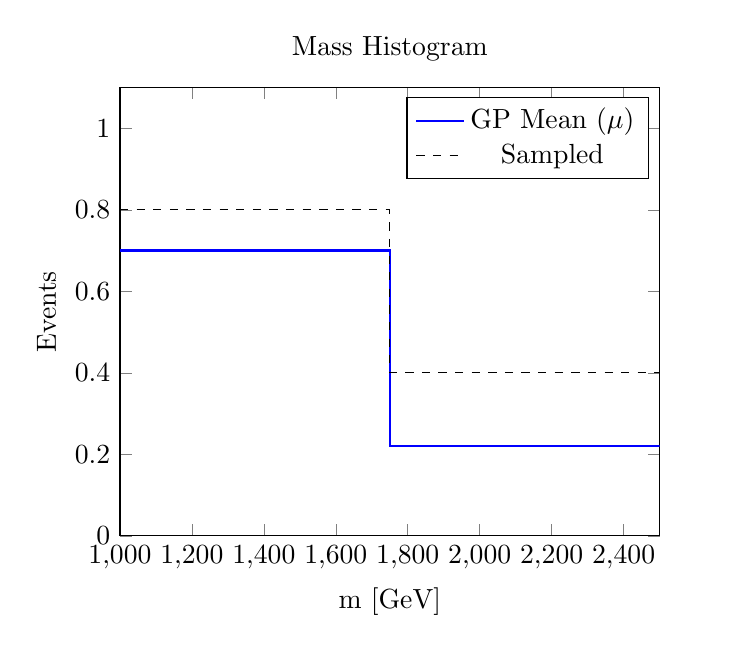
\begin{tikzpicture}
  \def\center{(axis cs: \meanOne,\meanTwo)}
  \begin{scope}
    \begin{axis}[
      ymin=0, ymax=1.1,
      xmin=1000, xmax=2500,
      xlabel={m [GeV]},
      ylabel={Events},
      title=Mass Histogram,
      nodes near coords={\node (plot-\coordindex) at (axis cs:
        \pgfkeysvalueof{/data point/x}, \pgfkeysvalueof{/data point/y}) {};}
      ]
      \addplot[blue, thick, const plot mark mid, domain=1000:2500, samples=2, mark=none] plot coordinates {(1000,\binOne) (2500,\binTwo)};
      \addplot[thin, dashed,const plot mark mid, domain=1000:2500, samples=2, mark=none] plot coordinates {(1000,\meanOne) (2500,\meanTwo)};
      \legend{GP Mean ($\mu$), Sampled}
    \end{axis}
  \end{scope}
\end{tikzpicture}
\end{document}
